%%%%%%%%%%%%%%%%%%%%%%%%%%%%%%%%%%%%%%%%%%%%%%%%%%%%%%%%%%%%%%%%%%%%%%%%%%%%%%%%
\section{Methodology}
\label{sec:methodology}
I propose two approaches to combine Gramatron and Nautilus. First, I wrote a script that pipelines their execution without modifying any internal implementation. This method is easy to implement, but it incurs overhead caused by starting AFLplusplus twice during fuzzing. This method also has the limitation of only being able to run Gramatron before Nautilus because Gramatron cannot take seeds from other mutators. The second method allows Gramatron and Nautilus to run alternately. I modified Gramatron's internal implementation by adding an automaton parser. Without any addition to Gramatron's source code, Gramatron and Nautilus cannot run together because Gramatron cannot parse seeds generated by Nautilus into automaton representations. Once Gramatron is able to obtain these representations, it can mutate seeds generated by other sources and thus run together with Nautilus in one AFLplusplus fuzzing campaign. 

\subsection{Tool Pipeline}
The pipeline approach to combining Gramatron and Nautilus is shown in \figref{tool-pipelining}.
\begin{figure}[h]
  \centering
  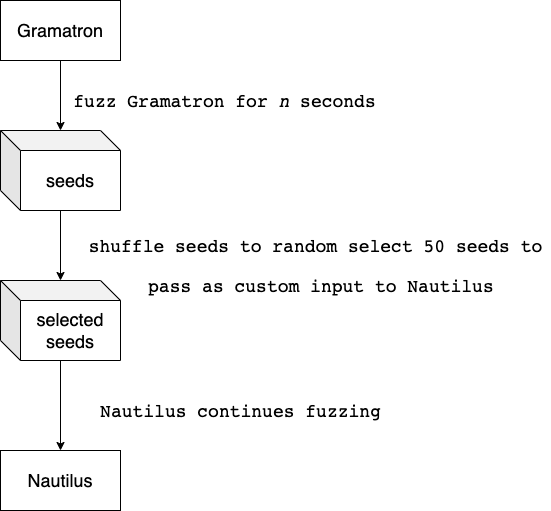
\includegraphics[scale=0.4]{images/pipeline.png}
  \caption{Tool Pipelining.}\label{tool-pipelining}
\end{figure}
The first step is to run Gramatron for a fixed amount of time that is determined heuristically. Then, shuffle the seeds generated by Gramatron to randomly select 50 seeds from the queue to feed into Nautilus. Nautilus can then continue fuzzing on top of Gramatron's generated results. 

This approach to combining the two fuzzers is easy to implement, but it suffers from the following problems.
\begin{enumerate}
    \item Additional time overhead is introduced because AFLplusplus is started twice in each fuzzing campaign. 
    \item The time used to fuzz Gramatron is determined heuristically. It is difficult to decide when is the right time to switch over to Nautilus. If Gramatron is run for too long, the crash might occur before Nautilus is even run, and we lose the benefit we could gain from Nautilus' localized search. On the other hand, if Gramatron is run for only a short time, most of the fuzz work would fall on Nautilus and we lose the benefit from Gramatron's aggressive mutator.
    \item The sequence of running Gramatron and Nautilus is fixed. 
\end{enumerate}

\subsection{Automaton Parser}
To enable Gramatron to accept seeds generated by other mutators, I implemented an automaton parser inside Gramatron. Internally, Gramatron keeps a data structure that stores the FSA representation of the input grammar. The process of learning the automaton walk is essentially a depth first search. The automaton learner parser in the following steps.
\begin{enumerate}
    \item Start from the starting state of the FSA.
    \item Start from the position in the input seed that hasn't been read so far, greedily match the content of the input seed with the symbols of the input language until the next symbol \texttt{s} in the input seed is found. \label{dfs-2}
    \item Iterate through all the out going edges connected to the current state. Each edge has a symbol associated with it as shown in \figref{example-fsa}. Multiple edges that represent the same symbol can be present, so different edges could be explored before the right one is found. If the current symbol \texttt{s} matches the an edge, advance to the state the edge links to and move the position in the input seed, record the edge taken and go to step \ref{dfs-2}. If no edge matches \texttt{s}, discard the current path. 
    \item If the end of the input seed is reached, check if the current state is the accepting state. If the path is accepted, return the current automaton walk. If not, discard the current path.
\end{enumerate}
After an input seed is parsed into an automaton walk, Gramatron would store the walk into a binary file for future reference.

\subsection{Integration inside AFLplusplus}
AFLplusplus has implemented the API that allows users to use one or more custom mutators. \figref{aflplusplus} shows how AFLplusplus works with both Gramatron and Nautilus.

\begin{figure}[]
  \centering
  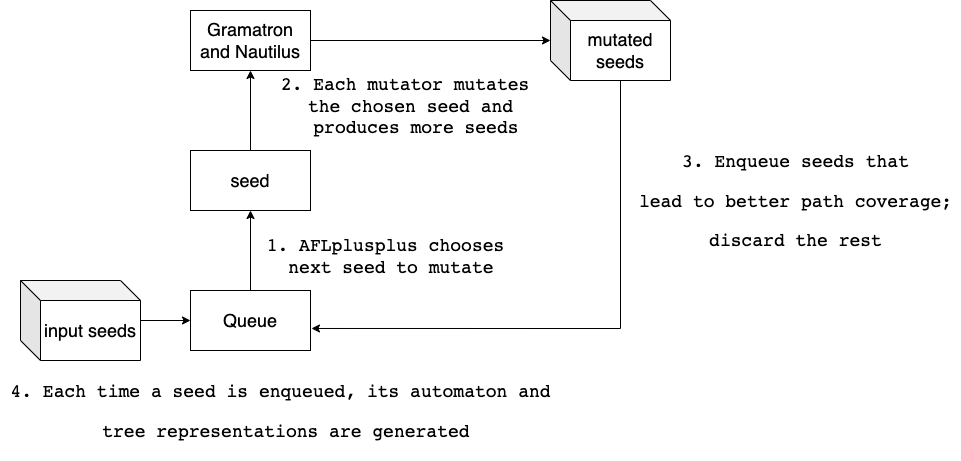
\includegraphics[scale=0.28]{images/AFLplusplus.png}
  
  \caption{AFLplusplus with both Gramatron and Nautilus.}\label{aflplusplus}
\end{figure}

The user would first provide a set of input seeds that comply with the input grammar. All the initial seeds are euqueued into AFLplusplus' internal queue. Every time a seed is enqueued, its automaton and tree representations are generated. During a fuzzing campaign, AFLplusplus first picks a seed from the queue to fuzz. Both Gramatron and Nautilus would be run on each seed to produce more seeds. AFLplusplus then inspects each new seed and enqueue the ones that lead to better path coverage. Since now Gramatron and Nautilus can read each other's seeds, this second method allows Gramatron and Nautilus to run alternately.


